% %%%%%%%%%%%%%%%%%%%%%%%%%%%%%%%%%%%%%%%%%%%%%%%%%%%%%%%%%%%%%%%%%%%%%%%%%%%%%%%
\documentclass[journal,letterpaper]{IEEEtran}
% include the list of acronyms, math commands and new commands used in this paper
% \usepackage[backend=bibtex,maxnames=2]{biblatex}
\usepackage[pdftex]{graphicx}
\usepackage[numbers]{natbib}
\bibliographystyle{IEEEtran} 
\usepackage{booktabs}
\usepackage{moreverb}
%\usepackage{titlesec}
%\usepackage[titletoc,toc,title]{appendix}
\usepackage{url}
\usepackage{amsmath}
\usepackage{multicol,lipsum}
\usepackage{mathtools}
\usepackage{cuted}
\usepackage{amsfonts}
\usepackage{multirow}
\usepackage{bm}
\usepackage{subfig}
\usepackage{color, colortbl}
\usepackage[colorlinks,bookmarksopen,bookmarksnumbered,citecolor=red,urlcolor=red]{hyperref}

\usepackage{enumitem}

\hypersetup
{
	pdftitle = {Orientation Control System: Enhancing Aerial Maneuvers for Quadrupedal Robots},
	pdfauthor = {Roscia, Cumerlotti, Del Prete, Semini, Focchi},
	pdfsubject = {Humanoids 2022 manuscript},
	pdfkeywords = {legged robots, aerial locomotion, and safe landing},
	pdftoolbar = true,
	colorlinks = true,
	linkcolor = black,
	citecolor = black,
	urlcolor = black,
}

\usepackage[usenames,dvipsnames]{xcolor}%\usepackage{xcolor,colortbl}
\definecolor{blue_iit}{RGB}{51,51,255}
\usepackage{algpseudocode}
\usepackage{algorithm}
\usepackage{glossaries}
\usepackage[tight]{units}
\usepackage[normalem]{ulem} % to strike out text, use: \sout{text}
\usepackage{cancel}
\definecolor{Gray}{gray}{0.9}
\usepackage{tensor} 
\usepackage{nicefrac}
%\usepackage{cleveref}
%\crefname{figure}{Fig.}{Fig.}
%\crefname{equation}{Eq.}{Eq.}
%\AtBeginDocument{%
%  \renewcommand{\crefpairconjunction}{,}%% instead of " and\nobreakspace"
%  \renewcommand{\crefmiddleconjunction}{,}% instead of ", "
%  \renewcommand{\creflastconjunction}{,}% instead of " and\nobreakspace"
%}

%\usepackage[backend=biber, sorting=none, style=ieee]{biblatex}
%\addbibresource{references/bibliography} 
\input{includes/acronyms.tex}
\input{includes/math_commands.tex}
\newcommand{\sref}[1]{Section~\ref{#1}}
%\newcommand{\eref}[1]{Eq.~(\ref{#1})}
\newcommand{\eref}[1]{(\ref{#1})}
\newcommand{\fref}[1]{Fig.~\ref{#1}}
\newcommand{\tref}[1]{Table~\ref{#1}}



%\newtheorem{Assumption}{Assumption}[section]
\newtheorem{assump}{Assumption}
\newtheorem{assumpB}{Assumption}
\renewcommand\theassump{1}
\renewcommand\theassumpB{2}
\newcommand{\assref}[1]{Assumption~\ref{#1}}



\newcommand{\AR}[1]{\textcolor{blue}{\textbf{aradulescu}: #1}}
\newcommand{\MF}[1]{\textcolor{red}{\textbf{mfocchi}: #1}}
\newcommand{\CS}[1]{\textcolor{violet}{\textbf{csemini}: #1}}
\newcommand{\SF}[1]{\textcolor{teal}{\textbf{sfahmi}: #1}}



\newcommand\BibTeX{{\rmfamily B\kern-.05em \textsc{i\kern-.025em b}\kern-.08em
T\kern-.1667em\lower.7ex\hbox{E}\kern-.125emX}}


\newcommand{\ie}{{i.e.},\ }
\newcommand{\eg}{{e.g.},\ }
\newcommand{\etal}{{\textit{et~al.}}\ }


\captionsetup[table]{labelsep=newline}
\captionsetup[table]{justification=centering}



\makeatletter
\newcounter{definition*}
\newenvironment{definition*}[1][htb]
{\renewcommand{\ALG@name}{Definition}% Update algorithm name
	\let\c@algocf\c@megaalgorithm% Update algorithm counter
	\begin{algorithm*}[#1]%
	}{\end{algorithm*}}
\makeatother

\makeatletter
\newcounter{definition}
\newenvironment{definition}[1][t]
{\renewcommand{\ALG@name}{Proposition}% Update algorithm name
	\let\c@algocf\c@megaalgorithm% Update algorithm counter
	\begin{algorithm}[#1]%
	}{\end{algorithm}}
\makeatother

\newcommand{\defref}[1]{Proposition~\ref{#1}}


%\usepackage[table]{xcolor}
\definecolor{sfahmi_blue}{RGB}{0.19,0.51,0.74}
%\definecolor{DarkGray}{RGB}{0.25,0.25,0.25}
%\definecolor{Gray}{RGB}{0.5,0.5,0.5}
%\definecolor{Red}{RGB}{1,0,0}
\definecolor{LightBlue}{RGB}{0.4,0.4,1}
\newcommand{\thickhline}{\noalign{\hrule height 0.8pt}}

\newcommand{\bmcolor}[1]{\textcolor{RoyalBlue}{\bm{#1}}}


\hypersetup{draft}
\makeglossaries

\title{Reaction Wheels: Enhancing Aerial Maneuvers for
	Legged Robots (Tentative)}
\author{Andrea Cumerlotti$^{1, \, 2}$, Francesco Roscia$^{2, \, 3}$, Michele Focchi$^{2, \, 4}$, Andrea Del Prete$^{1}$ and Claudio Semini$^2$
	\thanks{$^1$ Industrial Engineering Department (DII), University of Trento, Trento, Italy.
		
	$^2$ Dynamic Legged Systems (DLS) lab, Istituto Italiano di Tecnologia (IIT), Genoa, Italy.
	
	$^3$ Computer Science and Technology, Bioengineering, Robotics and Systems Engineering (DIBRIS), University of Genoa, Genoa, Italy.
	
	$^4$ Department of Information Engineering and Computer Science (DISI), University of Trento, Trento, Italy.

}}


\begin{document}
\maketitle
\thispagestyle{empty}
\pagestyle{empty}

\begin{abstract}%150-250 word abstract
Aerial motions represent a challenge for quadrupedal robots. They become inevitable to overpass obstacles that cannot be circumvent with standard locomotion gaits. In these cases, the robot must perform a leap to position itself on the obstruction or even flyover it. In this work we propose an orientation control system consisting on a couple of rotating and actuated masses (named flywheels or reaction wheels) for the lightweight open-source robot Solo12. Because of the conservation of angular momentum, their rotation can be adjusted to steer the robot base orientation even when there are no contacts with the ground. The axes of rotation of the flywheels are designed to be incident, allowing us to have a compact orientation control system that is capable of controlling both roll and pitch angles of the platform considering the different moment of inertia in the two directions. We proof the concept with simulation and experiments on the real robot.
\end{abstract}

\begin{IEEEkeywords}
	 
\end{IEEEkeywords}

\section{Introduction}\label{sec:introduction}
Legged locomotion is designed for traversing rough terrain.
Different types of gait, such as trot or crawl, have been developed to move quadrupedal robots. 
Thanks to the progress of the last two decades, robots become lighter and able to generate higher torques and forces at the joints, enabling the possibility of doing highly dynamic maneuvers.
Sometimes it is not possible to get around an obstacle with the gaits mentioned above, and jumps may be required. 

When the robot is in air, the \acrfull{com} moves on the ballistic trajectory, that is completely defined by the lift-off position and velocity. On the other hand, the base orientation can be changed exploiting the conservation of the system angular momentum. This means that it is possible to control the base angular velocity by changing the inertia of the robot, e.g., changing the joints configuration. 

Nevertheless, the majority of quadrupeds are designed to respect the massless leg assumption, resulting in limbs having small influence on the total angular momentum.


\subsection{Related Work}
Quadrupedal animals, like cats, can rearrange the tail and trunk to correct the orientation during a fall \cite{kane1969dynamical}.
% Tail
Many works use an additional link as a tail, like in \cite{chu2019null} and \cite{wenger2016frontal}.
This link rotates around an axis that does not pass through the robot \acrshort{com}: the distances between the axis of rotation and the \acrshort{com} of both trunk and tail allow to obtain large effect on the total angular momentum even with a small tail mass.
However, the placement of the additional link makes the resulting robot asymmetric. Moreover, due to its limited range of motion, a tail can be used only for a single jump, not for a repeated sequence \cite{johnson2012tail}.\annotation{Andrea me la spieghi?}

% Legs reconfig
It is possible to obtain a similar result by creating repetitive circular motions with the feet, like in \cite{hoffman2021exploiting} and \cite{kurtz2021mini}.

In the latter, authors proposes special heavy boots for Mini Cheetah and use a neural network to calculate online joint trajectory. However, this solution unnecessarily increases the inertia of the legs, complicating the locomotion problem.\annotation{trova un modo per dire che questa complicazione è data dalla massless assumption che non è più valida} 

% Gyros
Another option is to use a \acrfull{cmg}.
It consists of a wheel, spinning at a constant angular velocity inside two or three actuated gimbals.
Tilting the wheel's axes of rotation generates the gyroscopic torque.
This system is widespread in spacecrafts reorientation \cite{yoon2002spacecraft}, but less frequently exploited in robot locomotion, either wheeled \cite{brown1996single} or legged \cite{mikhalkov2021gyrubot}.
The \acrshort{cmg} presents interesting capabilities, but the presence of a pan-tilt \annotation{Andrea mi spieghi che intendi} unit to the drive the gyroscope makes it impractical to mount it on a small, lightweight robot.

% Reaction wheel
Reaction wheels represent an additional option for controlling the robot orientation.
Changing the angular velocity of a rotating mass attached to the trunk generates a torque that can reorient and stabilize the robot. Also this device is borrowed by spacecraft orientation \cite{oland2009reaction}, and it was sporadically investigated in legged locomotion, both for bipeds \cite{Brown2016}  \cite{xiong2020sequential} and quadrupeds \cite{kolvenbach2019towards}, \cite{vasilopoulos2016quadruped}.
Compared with tails, reaction wheels do not have position limit, and since it rotates around its center of mass, its angular momentum results holonomic \cite{machairas2015quadruped}.\annotation{Andrea mi spieghi che intendi}
To get a fast response, it is necessary to have an abrupt change in the reaction wheel angular velocity (angular acceleration).
Using a brake avoids the employment of a motor able to deliver higher torques \cite{gajamohan2012cubli}, keeping the system compact: the motor speeds up slowly the reaction wheel, and when a reorientation is required, the break stops its spin.
Since the effect of the break is unidirectional, it is possible to generate a rotation of the base only in the opposite direction of the reaction wheel angular velocity.

\subsection{Proposed Approach and Contribution}
In this work, we present an \acrfull{ocs} based on two flywheels, mounted on the trunk of the quadruped Solo12 \cite{grimminger2020open}. In order to control roll and pitch orientations with a compact device, the axes of rotation are set to be incident, creating an angle that balances the effect in both the directions. 
Flywheels can correct orientation errors due to disturbances during the flight and inaccuracies in to the angular momentum achieved at the lift-off (e.g., given by tracking issues and non-idealities). 
They enable the robot to land with a desired angular velocity (possibly zero) and orientation.
In addition, they can enhance the landing phase by significantly reducing oscillations.  
The presence of these additional joints, whose only function is to control the orientation, gives the possibility to relieve the effort of the legs.
In more complex scenarios, like for a somersault, legs and flywheels can work in parallel to achieve a rotation angle larger than the one achievable only with legs (e.g., due to torque limitation). Furthermore, the \acrshort{ocs} can also be exploited to stabilize dynamic gaits, compensating for trunks oscillation.

\subsection{Outline}
% 

\section{Background}
The starting point for any \acrshort{ocs} is the Euler's equation. For any mechanical system, the time derivative of the angular momentum computed with the respect of with a reference point $O$ fixed in an inertial frame equals
the resultant torque with respect to the same reference point:
\begin{equation}
	\dot{\bm{L}} = \sum_i \bm{M}_i
\end{equation}
When the external moment applied to the system is zero, Euler’s equation simplifies in
\begin{equation}
\dot{\bm{L}} = 0 \quad \Rightarrow \quad \bm{L}(t) = const.
\end{equation}
which is known as conservation of angular momentum.
Referring to legged robots, this condition occurs whether the system is not in contact with the ground or other objects, e.g., during a fall or the flight phase of a jump.
In the case, it is possible to change the angular velocity of the base, changing the joints velocities, as a result of the \textit{non-holonomy} of the angular momentum \cite{Wieber16}: if the angular momentum of a certain body changes, the one of the others must modify to maintain the total sum constant.

\section{\acrshort{ocs} Design}
We want to control simultaneously the robot roll and pitch orientation.
To accomplish this task, the reaction wheels' contribution to the total angular momentum should lie on both $x$- and $y$-axes of the base frame, see Fig. \ref{fig:angVel}. 
To remove unnecessary complications, we design two symmetrical modules. The axes of rotation of the left and right wheel, identified in the base reference frame with the unit vectors $\hat{\bm{a}}_l$ and $\hat{\bm{a}}_r$\annotation{$\hat{\bm{a}}$ sta per axis, se non ci piace si può trasformare in $\hat{\bm{c}}$}, are set to be incident, spanning a plane parallel to the $xy-$ plane of the base reference frame. We denote with $\alpha \leq \pi/2$ the non-negative angle between the wheels'axes of rotation and the robot lateral direction\annotation{I suggest to call $\alpha$ incident angle}. As long as the matrix
\begin{equation}
	\bm{C} = 
	\left[ \begin{array}{cc}
	\hat{\bm{a}}_l & \hat{\bm{a}}_r
	\end{array} \right] = 
	\left[ \begin{array}{cc}
	\sin(\alpha) & \sin(\alpha) \\
	-\cos(\alpha) & \cos(\alpha) \\
	0 & 0
	\end{array} \right]
\end{equation}
is full column rank, it is possible to control both roll and pitch angles. If $\alpha = 0$, the roll results to be uncontrollable through the \acrshort{ocs}; otherwise, if $\alpha = \pi/2$, the pitch is not uncontrollable.
%
%\subsection{Inertia Selection}
%n order to find the inertia necessary to comply with the requirements of the orientation control system, some analyses are performed with the “Elroy’s Beanie” shown in figure \ref{fig:elroy-beanie}.
%This model consists of two bodies connected with a revolute joint on their Center of Mass (CoM).
%One of the bodies represents the robot (inertia $I_r$), simplified as a single rigid body, and the other one the flywheel (inertia $I_{fw}$).
%I perform the analysis for only one flywheel and only then extend the results to two bodies.
%\begin{figure}[H] 
%	\centering
%	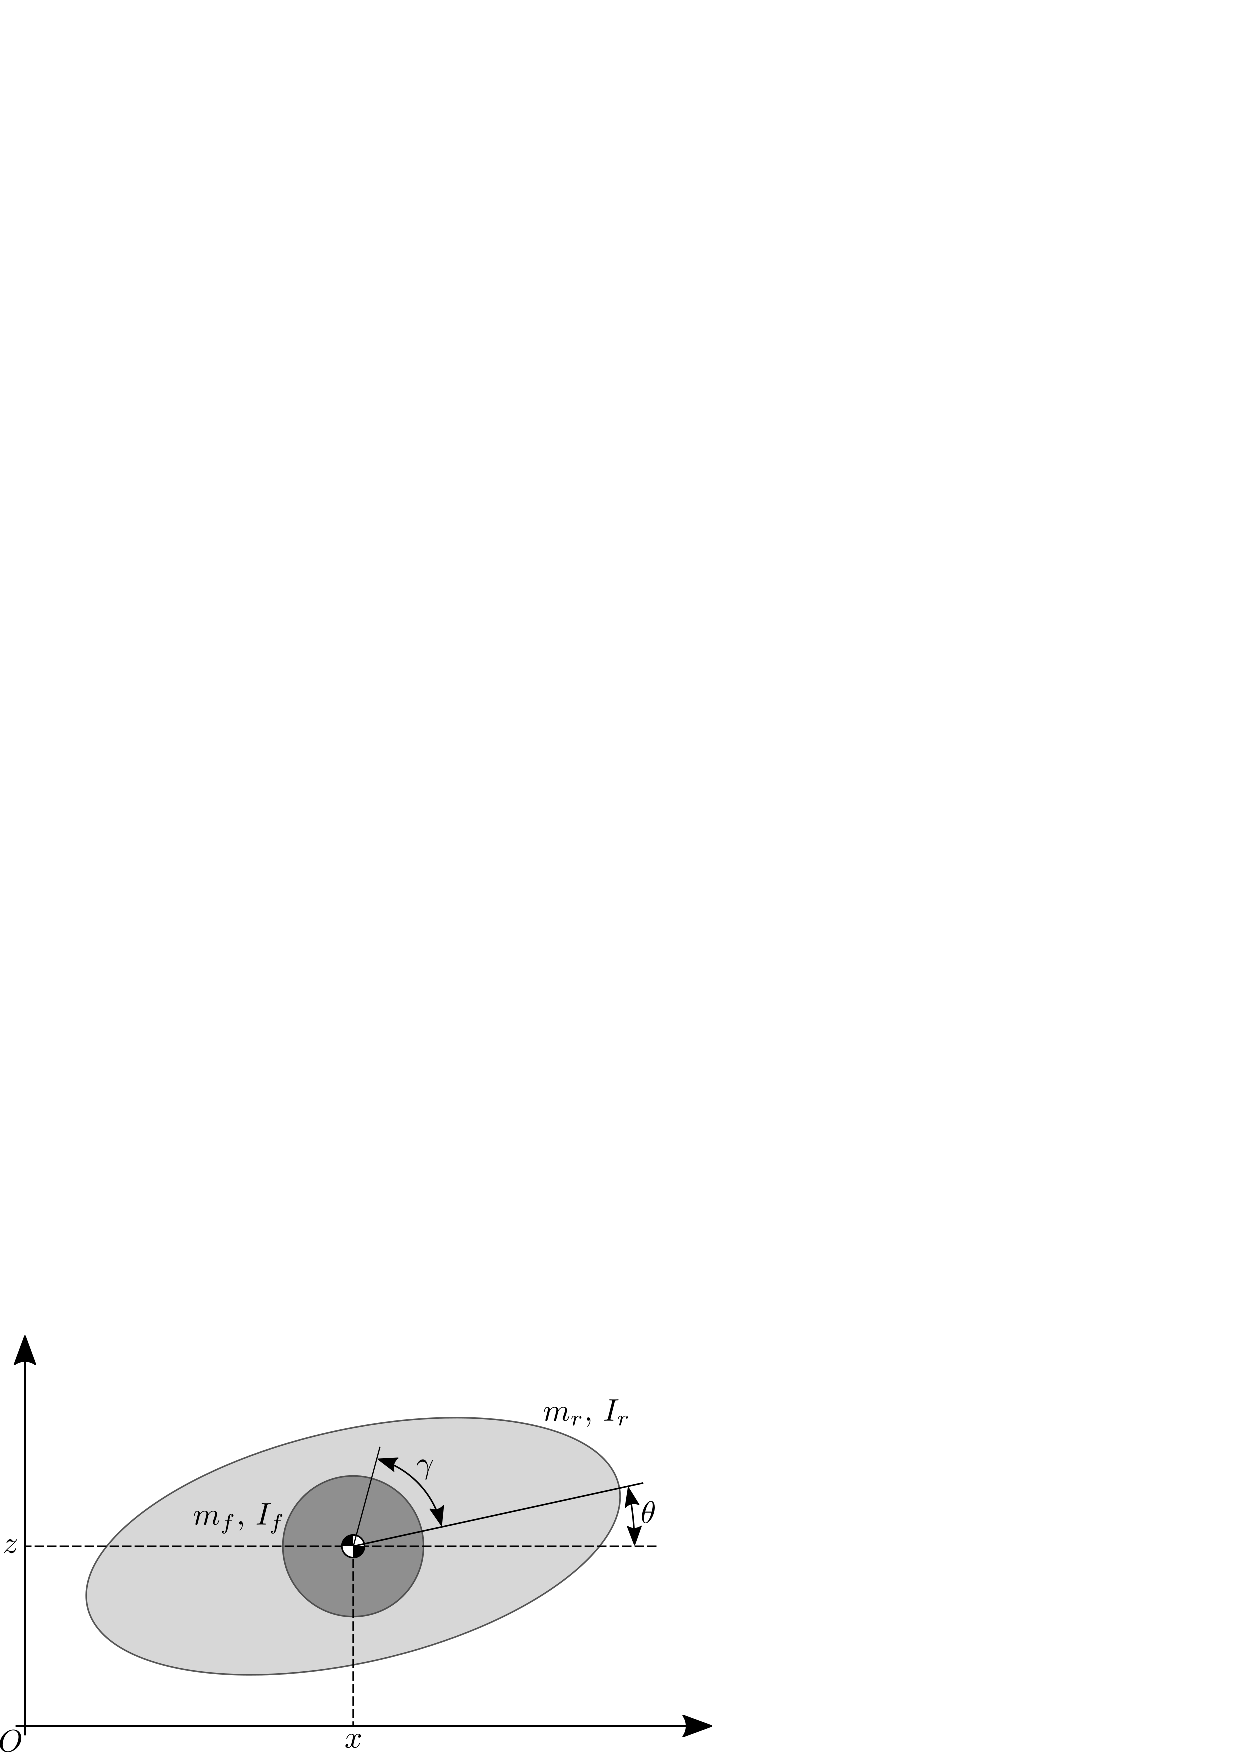
\includegraphics[height=5.9cm]{Images/Flywheel_System_Design/elroys-beanie.pdf}
%	\caption{Schematic representation of the Elroy's Beanie model used for the preliminary analysis of the pitch motion.}
%	\label{fig:elroy-beanie}
%\end{figure}
%\noindent
%The angular momentum $L$ of this system can be written as
%\begin{equation}\label{eq:ang_mom_elroy}
%L = \left(I_r + I_{fw}\right)\dot{\theta} + I_{fw}\dot{\gamma}
%\end{equation}
%in which $I_r$ is the $I_{yy}$ component of the centroidal inertia matrix of the robot and $I_{fw}$ is composed by both the reaction wheels inertia of the along their axis of rotation, $\dot{\theta}$ and $\dot{\gamma}$ correspond respectively to the pitch-rate and angular speed of the wheels.
%I employed the only the $I_{yy}$ component because, it gives the information about the pitch rotation.
%The other elements of the tensor of inertia that affect the pitch, such as $I_{yx}$ and $I_{yz}$, are not considered since they are negligible with the respect to  $I_{yy}$.
%Using the $I_{xx}$ component of the centroidal inertia matrix instead of the $I_{yy}$ allows us to perform the the same analysis as below for the roll rotation.
%In this case, the variable $\theta$ should be substitute by $\phi$, the roll angle.
%Under the condition of conservation of the angular momentum \ref{sec:cons_ang_mom} it is possible to estimate of the lower bound for $I_{fw}$ to get a desired angular velocity of the main body $\dot{\theta}_{des}$.
%Assuming that at the lift-off the reaction wheels are not spinning ($\dot{\gamma}_{lo} = 0$), the angular momentum is $L_{lo} = \left(I_r + I_{fw}\right)\dot{\theta}_{lo}$, in which $\dot{\theta}_{lo}$ is the base pitch rate at lift-off. This value does not change for the whole duration of the flight.
%The minimum inertia necessary to reach $\dot{\theta}_{des}$ is obtained when the flywheels rotate at their maximum speed. For higher inertia it is sufficient a smaller angular velocity:
%\begin{equation}
%I_{fw} = I_r \frac{\dot{\theta}_{lo} - \dot{\theta}_{des}}{\dot{\theta}_{des} + \dot{\gamma}_{max} - \dot{\theta}_{lo}} \ .
%\end{equation}
%The variable $\dot{\gamma}_{max}$ is the maximum motor speed that correspond to $5000 \ \mathrm{RPM}$ ( $523.6 \ \mathrm{rad/s}$).
%In figure \ref{fig:pre_ana_kin} the results for different initial and desired angular velocities are reported.
%It is evident that high inertia is required when the inertial and the desired angular velocity are opposite.
%Usually, this condition is avoided thanks to a good thrusting phase.
%\begin{figure}[H]
%	\centering
%	\includegraphics[width=0.7\textwidth]{Images/Flywheel_System_Design/Inertia_selection_by_kinematic_limits.eps}
%	\caption{Minimum inertia necessary to obtain the angular velocity $\dot{\theta}_{des}$ starting with different lift-off $\dot{\theta}_{lo}$ conditions.}
%	\label{fig:pre_ana_kin}
%\end{figure}
%
%The kinematic model employed before has not considered the transient to reach the desired angular speed.
%For this reason, the dynamical model of the "Elroy's Beanie" mechanism is derived.
%The dynamics of this system is obtained with the Lagrangian method.
%To calculate the Lagrangian $L$ it is necessary to compute the kinetic energy $K$ and the potential energy $U$.
%In this quantities must be included also the translation part, therefore are used the masses of the bodies, $m_r$ and $m_{fw}$, and the position of the CoM, $x$ and $z$. 
%\begin{equation*}
%K = \frac{1}{2}\left(m_r + m_{fw}\right)\left(\dot{x}^2 + \dot{z}^2\right) + \frac{1}{2}I_r \dot{\theta}^2 + \frac{1}{2} I_{fw} \left(\dot{\theta} + \dot{\gamma}\right)^2
%\end{equation*}
%\begin{equation*}
%U = \left(m_r + m_{fw}\right) g z 
%\end{equation*}
%\begin{equation}
%\begin{split}\label{eq:lagrangian}
%L &= K - U\\
%&= \frac{1}{2}\left(m_r + m_{fw}\right)\left(\dot{x}^2 + \dot{z}^2\right) + \frac{1}{2}\left(I_r + I_{fw}\right)\dot{\theta}^2 + \frac{1}{2} I_{fw}\dot{\gamma}^2 + I_{fw} \dot{\theta}\dot{\gamma} - \left(m_r + m_{fw}\right) g z
%\end{split}
%\end{equation}
%\begin{equation}\label{eq:LagToEqMo}
%\frac{\partial L}{\partial \mathbf{q}} - \frac{d}{dt}\left(\frac{\partial L}{\partial \dot{\mathbf{q}}}\right) =  \boldsymbol{\tau}
%\end{equation}
%From the Lagrangian $L$ is possible to derive the equation of motion using \ref{eq:LagToEqMo}, in which $\mathbf{q} = \left[\begin{array}{cccc} x & z & \theta & \gamma \end{array}\right]^T$ are the generalized coordinates and $ \boldsymbol{\tau} $ are the generalized forces applied to the bodies.
%In this particular case, it is analysed the flight phase in which are not applied external forces or torques, apart from the flywheels' ones.
%Then we can set $\boldsymbol{\tau} = \left[\begin{array}{cccc} 0 & 0 & 0 & \tau_m \end{array}\right]^T$, in which $\tau_m$ is the direct-drive torque applied by the motor that control the flywheel.
%The resulting equation of motion are
%\begin{equation}\label{eq:EqOfMo}
%\left[\begin{array}{cccc}
%m_r + m_{fw} & 0 & 0 & 0\\
%0 & m_r + m_{fw} & 0 & 0\\
%0 & 0 & I_r+I_{fw} & I_{fw}\\
%0 & 0 & I_{fw} & I_{fw} \\
%\end{array}\right]
%\left[\begin{array}{c}
%\ddot{x} \\ \ddot{y} \\ \ddot{\theta} \\ \ddot{\phi} \\
%\end{array}\right] + 
%\left[\begin{array}{c}
%0 \\ \left(m_r + m_{fw}\right) g \\ 0 \\ 0 \\
%\end{array}\right] = 
%\left[\begin{array}{c}
%0 \\ 0 \\ 0 \\ \tau \\
%\end{array}\right] \ .
%\end{equation}
%To obtain the values of $\mathbf{q}$, the differential equations are integrated using Runge-Kutta 4th order method.
%From \ref{eq:EqOfMo}, we can see that the linear and the angular dynamic are decoupled.
%The linear part, which corresponds to the well-known motion of a projectile, is used to calculate the time of flight.
%I suppose that the robot lands on a flat surface at height zero.
%The landing is estimated when the CoM reach the height of $0.23 \ \mathrm{m}$ (distance between CoM and ground in homing configuration) with a negative velocity.
%This information is needed to understand the maximum time in which the reorientation maneuver must be concluded.
%The linear dynamics can be neglected, imposing a fixed time constraint based on the specification of the duration of the flight phase to $1 \ \mathrm{s}$.
%
%The inertia of the reaction wheels can be chosen minimizing the work done by the motor to perform a reorientation maneuver. In particular, the task analyzed was a rotation of the main body of $30^\circ$ ($\simeq 0.5 \ \mathrm{rad}$) in the time  $t_f = 1 \ \mathrm{s}$.
%A fifth-order polynomial generates the desired trajectory of the pitch of the robot that performs the rotation starting and finishing with zero angular velocity and acceleration.
%In order to track the trajectory, we assume that we use a proportional and derivative (PD) controller.
%The gains $k_p$ and $k_d$ are chosen to obtain a small settling time avoiding overshoots.
%\begin{equation*}
%\tau_m(t) = k_p \left(\theta_{des}(t) - \theta(t)\right) + k_d \left(\dot{\theta}_{des}(t) - \dot{\theta}(t)\right)
%\end{equation*}
%To select the inertia we intend to perform an optimization where we minimize the integral of the motor power absolute value, during the reorientation task.
%The inertia $I_r$ affects the dynamics of the system and then modifies the evolution of $\tau_m(t)$ and $\dot{\gamma}(t)$ during the task.
%\begin{equation*}
%\min_{I_r} \int_{0}^{t_f} |\tau_m(t)\dot{\gamma}(t)| \,dt
%\end{equation*}
%In figure \ref{fig:inertia_vs_energy} are shown the values of the work done by the motors,for correcting both roll and pitch of Solo12. The dissipated energy is monotonically decreasing in the flywheel's inertia.
%From the results, it is evident that there is not a local minimum and the optimal value for the inertia $I_{fw}$ is the greatest as possible.
%\begin{figure}[H]
%	\centering
%	\includegraphics[height=6cm]{Images/Flywheel_System_Design/Inertia_vs_energy.eps}
%	\caption{Work done by the motor $W_m$ using different values of inertia $I_{fw}$ for the reaction wheel  during a reorientation manoeuvrer of $30^\circ$ in $1s$.
%		The $x$-axis is in logarithmic scale to show a wide spectrum of inertias.
%		The results of the roll (in red) and pitch (in blue) are difference due to the different value of $I_r$, indeed the components of the centroidal inertia of the robot $I_{xx}$ and $I_{yy}$ are very different.}
%	\label{fig:inertia_vs_energy}
%\end{figure}
%
%\noindent
%With the same analysis, I investigated whether the inclusion of a gearbox between the motor and the reaction wheel would bring some benefits.
%The dynamical model is modified including the gearbox, with a gear reduction ratio $n$.
%In this case, the motor angular velocity and the one of the reaction wheel are no more equal.
%I continue to use $\gamma$ to define the motor angle, while the one of the flywheel is $\gamma / n$.
%The torque applied at the reaction wheel is the torque of the motor magnified by a a factor $n$.
%\begin{equation}\label{eq:EqOfMo_wGB}
%\left[\begin{array}{cccc}
%m_r + m_{fw} & 0 & 0 & 0\\
%0 & m_r + m_{fw} & 0 & 0\\
%0 & 0 & I_r+I_{fw} & I_{fw}/n\\
%0 & 0 & I_{fw} & I_{fw}/n \\
%\end{array}\right]
%\left[\begin{array}{c}
%\ddot{x} \\ \ddot{y} \\ \ddot{\theta} \\ \ddot{\gamma} \\
%\end{array}\right] + 
%\left[\begin{array}{c}
%0 \\ \left(m_r + m_{fw}\right) g \\ 0 \\ 0 \\
%\end{array}\right] = 
%\left[\begin{array}{c}
%0 \\ 0 \\ 0 \\ n\tau_m \\
%\end{array}\right]
%\end{equation}
%The problem of minimization is modified including the gear reduction ratio as a decision variable.
%\begin{equation}
%\min_{I_r,\, n} \int_{0}^{t_f} |\tau_m(t)\dot{\gamma}(t)| \,dt
%\end{equation}
%The results, in figure \ref{fig:gearbox_vs_energy}, point out that the presence of a gearbox with a reduction ratio as great as possible results in a minimization of the energy used to perform the reorientation maneuvers.
%The simulation of the task points out that adding the gearbox reduce the tracking error, but decrease of a factor $1/n$ the maximum speed of the motor.
%I decide to maintain the value of $n = 1$ (without gearbox), to avoid the saturation of the motor velocity during a common task and because using a greater value do not comport a relevant decrease in energy.
%\begin{figure}[H]
%	\centering
%	\includegraphics[height=6cm]{Images/Flywheel_System_Design/gearbox_vs_energy.eps}
%	\caption{Work done by the motor $W_m$ using different values of reduction ratio $n$ for the reaction wheel  during a reorientation manoeuvrer of $30^\circ$ in $1s$.
%		The $x$-axis is in logarithmic scale to show a wide spectrum of inertias.
%		The results of the roll (in red) and pitch (in blue) are difference due to the different value of $I_r$, indeed the components of the centroidal inertia of the robot $I_{xx}$ and $I_{yy}$ are very different.}
%	\label{fig:gearbox_vs_energy}
%\end{figure}
%\subsection{Incident Angle Selection}
%
%Let $\bm{I}^r = \mathrm{diag}{I^r_xx, \, I^r_yy, \, I^r_zz}$ be the inertia tensor of the robot in nominal configuration, expressed at its \acrshort{com}. The angle $\alpha$ that allows to maximize the joint contribution to the angular momentum on both the directions is 
\begin{figure}
	\centering
	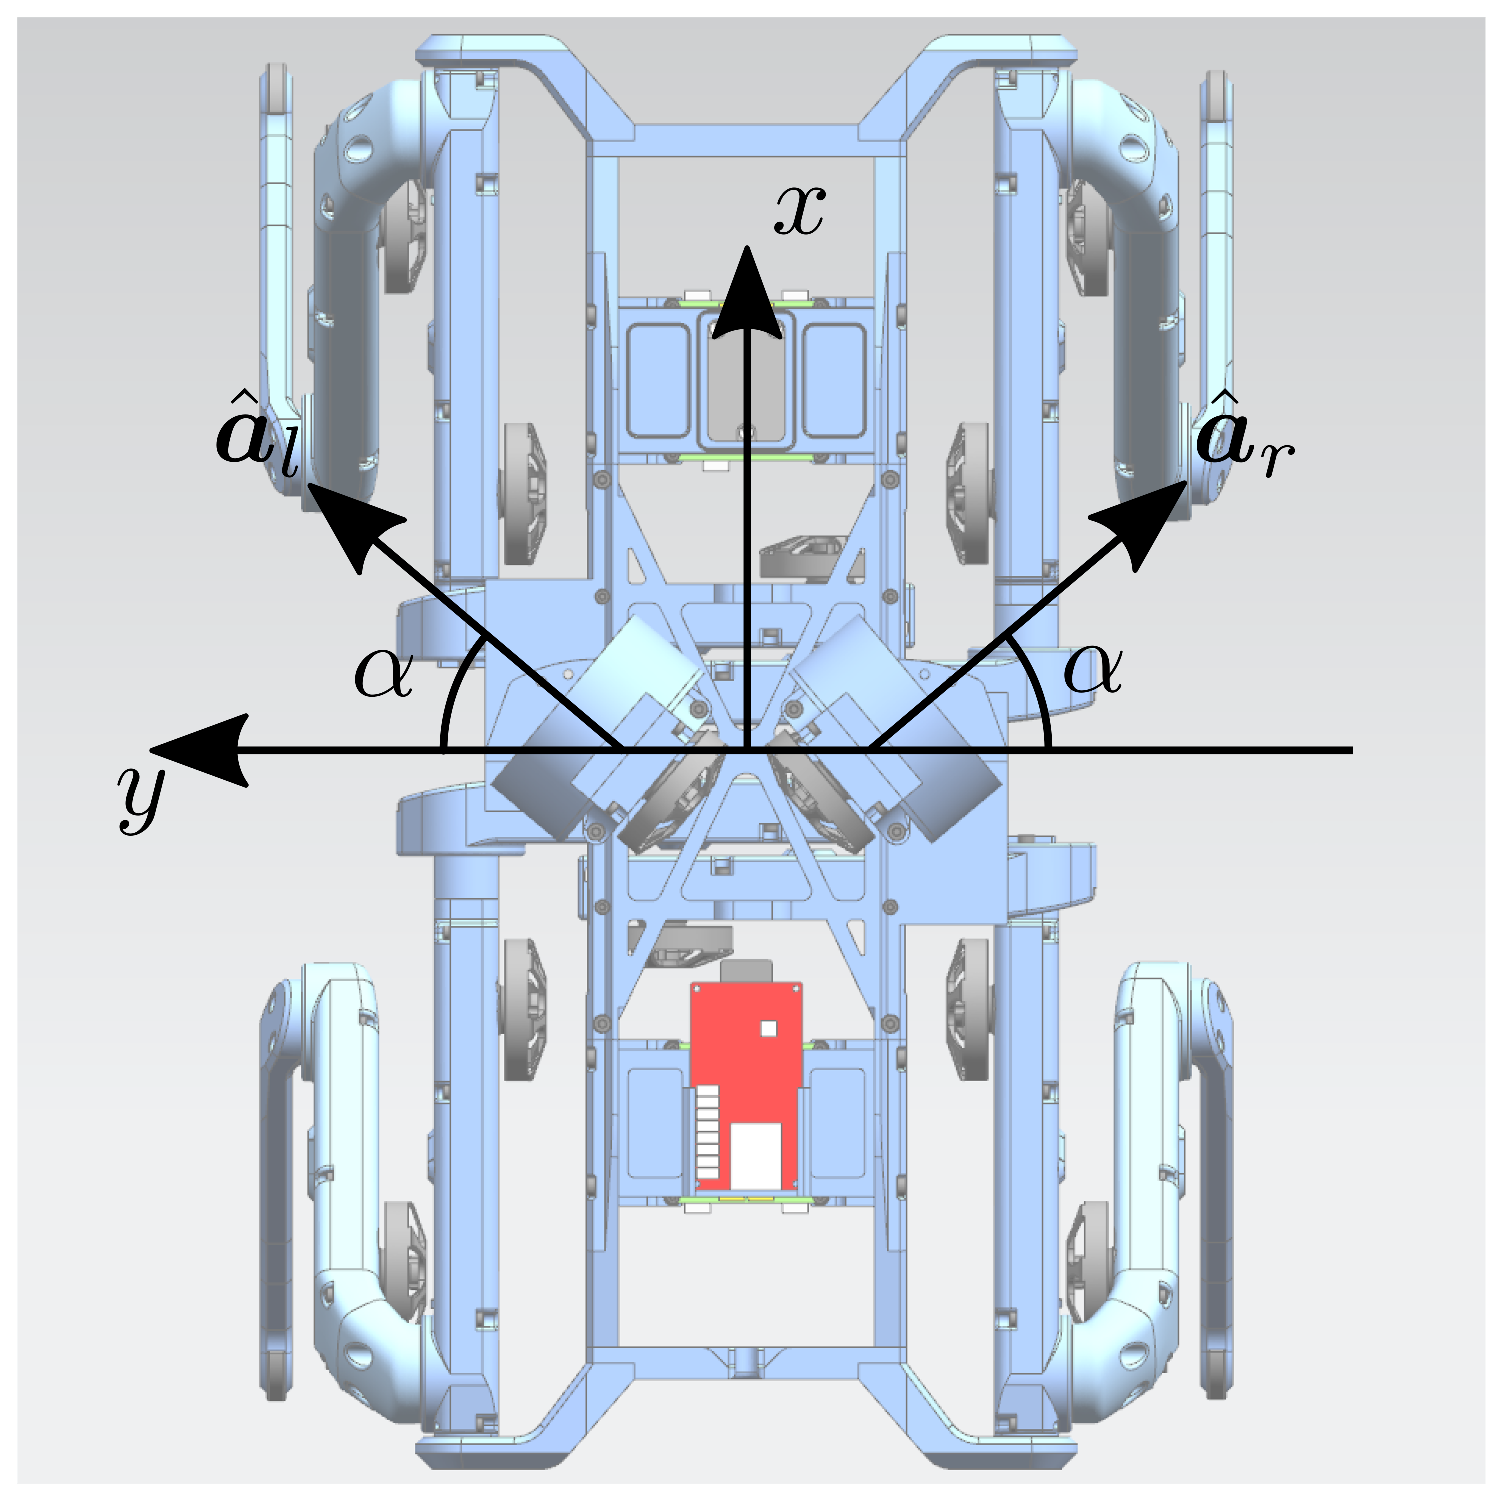
\includegraphics[width=0.7\linewidth]{figures/angular_velocities.eps}
	\caption{Representation of the flywheels rotation axes, seen from the top of the robot}
	\label{fig:angVel}
\end{figure}
\section{Conclusions}
\label{sec:conclusion}

\small
\section*{Acknowledgements}	



\printbibliography
\end{document}